\documentclass[]{article}
\usepackage{lmodern}
\usepackage{amssymb,amsmath}
\usepackage{ifxetex,ifluatex}
\usepackage{fixltx2e} % provides \textsubscript
\ifnum 0\ifxetex 1\fi\ifluatex 1\fi=0 % if pdftex
  \usepackage[T1]{fontenc}
  \usepackage[utf8]{inputenc}
\else % if luatex or xelatex
  \ifxetex
    \usepackage{mathspec}
  \else
    \usepackage{fontspec}
  \fi
  \defaultfontfeatures{Ligatures=TeX,Scale=MatchLowercase}
\fi
% use upquote if available, for straight quotes in verbatim environments
\IfFileExists{upquote.sty}{\usepackage{upquote}}{}
% use microtype if available
\IfFileExists{microtype.sty}{%
\usepackage{microtype}
\UseMicrotypeSet[protrusion]{basicmath} % disable protrusion for tt fonts
}{}
\usepackage[margin=1in]{geometry}
\usepackage{hyperref}
\hypersetup{unicode=true,
            pdftitle={Griffiths et al},
            pdfborder={0 0 0},
            breaklinks=true}
\urlstyle{same}  % don't use monospace font for urls
\usepackage{graphicx,grffile}
\makeatletter
\def\maxwidth{\ifdim\Gin@nat@width>\linewidth\linewidth\else\Gin@nat@width\fi}
\def\maxheight{\ifdim\Gin@nat@height>\textheight\textheight\else\Gin@nat@height\fi}
\makeatother
% Scale images if necessary, so that they will not overflow the page
% margins by default, and it is still possible to overwrite the defaults
% using explicit options in \includegraphics[width, height, ...]{}
\setkeys{Gin}{width=\maxwidth,height=\maxheight,keepaspectratio}
\IfFileExists{parskip.sty}{%
\usepackage{parskip}
}{% else
\setlength{\parindent}{0pt}
\setlength{\parskip}{6pt plus 2pt minus 1pt}
}
\setlength{\emergencystretch}{3em}  % prevent overfull lines
\providecommand{\tightlist}{%
  \setlength{\itemsep}{0pt}\setlength{\parskip}{0pt}}
\setcounter{secnumdepth}{0}
% Redefines (sub)paragraphs to behave more like sections
\ifx\paragraph\undefined\else
\let\oldparagraph\paragraph
\renewcommand{\paragraph}[1]{\oldparagraph{#1}\mbox{}}
\fi
\ifx\subparagraph\undefined\else
\let\oldsubparagraph\subparagraph
\renewcommand{\subparagraph}[1]{\oldsubparagraph{#1}\mbox{}}
\fi

%%% Use protect on footnotes to avoid problems with footnotes in titles
\let\rmarkdownfootnote\footnote%
\def\footnote{\protect\rmarkdownfootnote}

%%% Change title format to be more compact
\usepackage{titling}

% Create subtitle command for use in maketitle
\newcommand{\subtitle}[1]{
  \posttitle{
    \begin{center}\large#1\end{center}
    }
}

\setlength{\droptitle}{-2em}
  \title{Griffiths et al}
  \pretitle{\vspace{\droptitle}\centering\huge}
  \posttitle{\par}
  \author{}
  \preauthor{}\postauthor{}
  \date{}
  \predate{}\postdate{}


\begin{document}
\maketitle

\subsection{R Markdown}\label{r-markdown}

\begin{verbatim}
##     date             site sample.id quadrat.location macrophyte.id
## 1 6/7/15 choked_edge_wolf         a             -160       zostera
## 2 6/7/15 choked_edge_wolf         b              -40       zostera
## 3 6/7/15 choked_edge_wolf         c              -80       zostera
## 4 6/7/15 choked_edge_wolf         d             -120       zostera
## 5 6/7/15 choked_edge_wolf         e                0       zostera
## 6 6/7/15 choked_edge_wolf         f               40       zostera
##   number.shoots.quadrat foil.weight foil.wet.macro.weight
## 1                     7        8.29                100.16
## 2                    12        7.90                151.56
## 3                     9        7.90                154.93
## 4                     7        8.35                129.63
## 5                     8        8.20                113.37
## 6                    10        7.60                147.81
##   foil.dry.macro.weight total.dry.macro.weight microepiphyte.weight
## 1                 20.55                  12.26                   NA
## 2                 26.98                  19.08                   NA
## 3                 29.48                  21.58                   NA
## 4                 25.67                  17.32                   NA
## 5                 22.35                  14.15                   NA
## 6                 31.53                  23.93                   NA
##   macroepiphyte.weight drift.seaweed.weight rooted.seaweed.weight
## 1                 4.88                 5.93                    NA
## 2                 2.98                12.19                    NA
## 3                 6.87                 7.27                    NA
## 4                 7.08                 9.72                    NA
## 5                 4.36                 9.64                    NA
## 6                 1.45                 6.30                    NA
##   rooted.phylospadix notes
## 1                       NA
## 2                       NA
## 3                       NA
## 4                       NA
## 5                       NA
## 6                       NA
\end{verbatim}

\begin{verbatim}
## Warning: running command ''/usr/bin/otool' -L '/Library/Frameworks/
## R.framework/Resources/modules/R_de.so'' had status 1
\end{verbatim}

FIGURE 1: SPATIAL TRENDS IN SMITHORA LOAD

Figure 1C: Smithora load in edge v interior sites\\
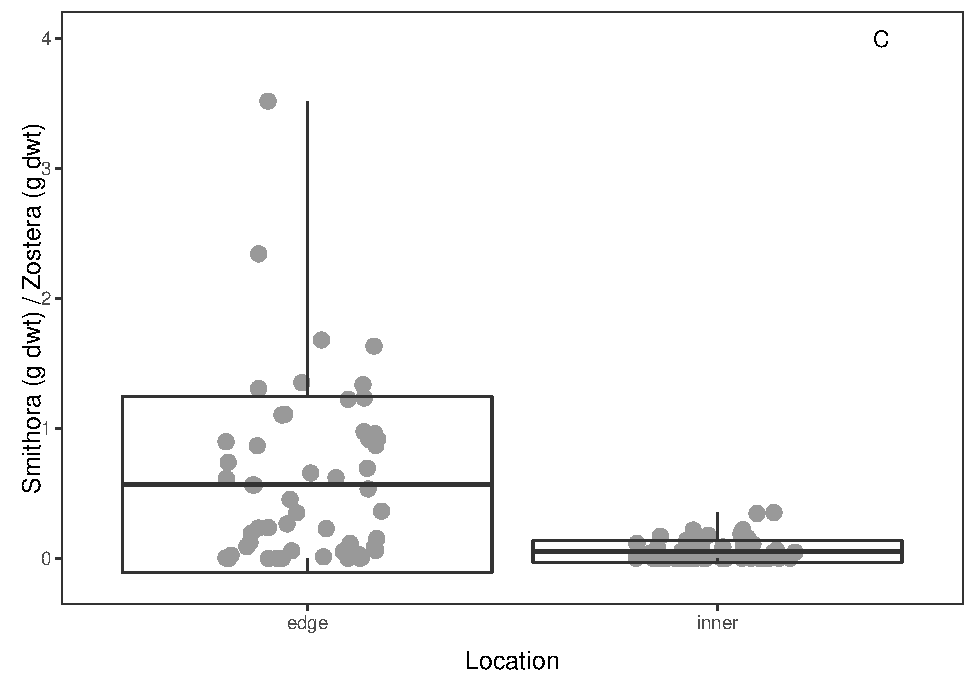
\includegraphics{Griffiths_et_al_analyses_and_figures_files/figure-latex/unnamed-chunk-4-1.pdf}

Analysis

\begin{verbatim}
## Model selection table 
##         (Int) grp.y sit grp.y:sit df   logLik  AICc delta weight
## mod3.2 -1.498     +   +         +  9 -193.141 406.0  0.00      1
## mod3.1 -1.597     +                3 -214.592 435.4 29.42      0
## Models ranked by AICc(x)
\end{verbatim}

\begin{verbatim}
## [1] 0.3746764
\end{verbatim}

\begin{verbatim}
## [1] 0.0220294
\end{verbatim}

Monitoring data (started with our data, but there isn't an inner site
here, really\ldots{})

\begin{verbatim}
## Warning: running command ''/usr/bin/otool' -L '/Library/Frameworks/
## R.framework/Resources/modules/R_de.so'' had status 1
\end{verbatim}

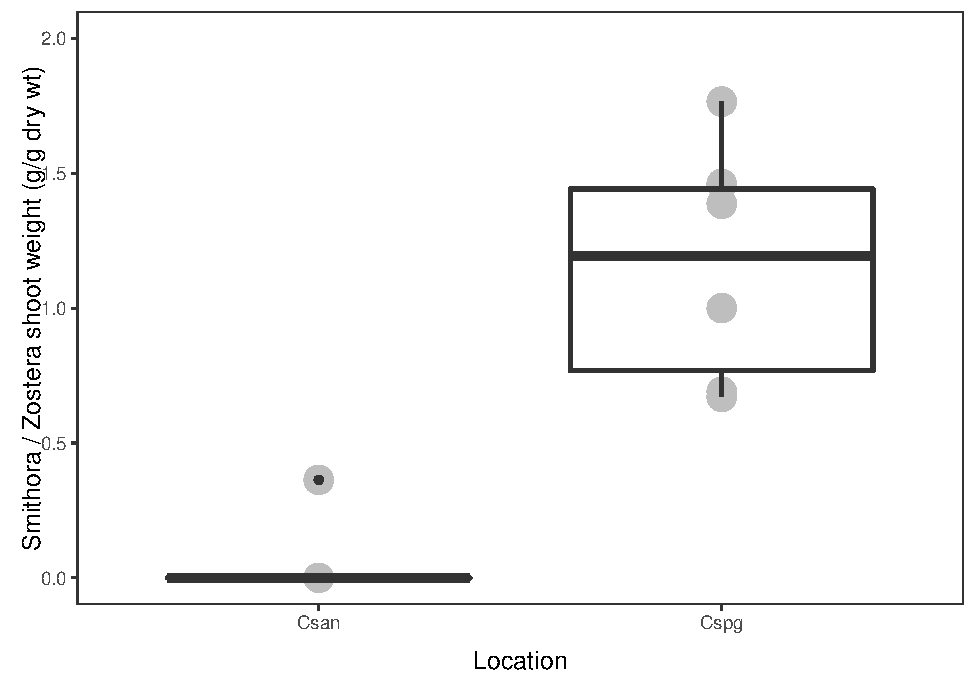
\includegraphics{Griffiths_et_al_analyses_and_figures_files/figure-latex/unnamed-chunk-6-1.pdf}
FIGURE 2: ZOSTERA, SMITHORA and GRAZER ABUNDANCE at transplant sites
before experiment A) Shoot density (moved to supplementary material)
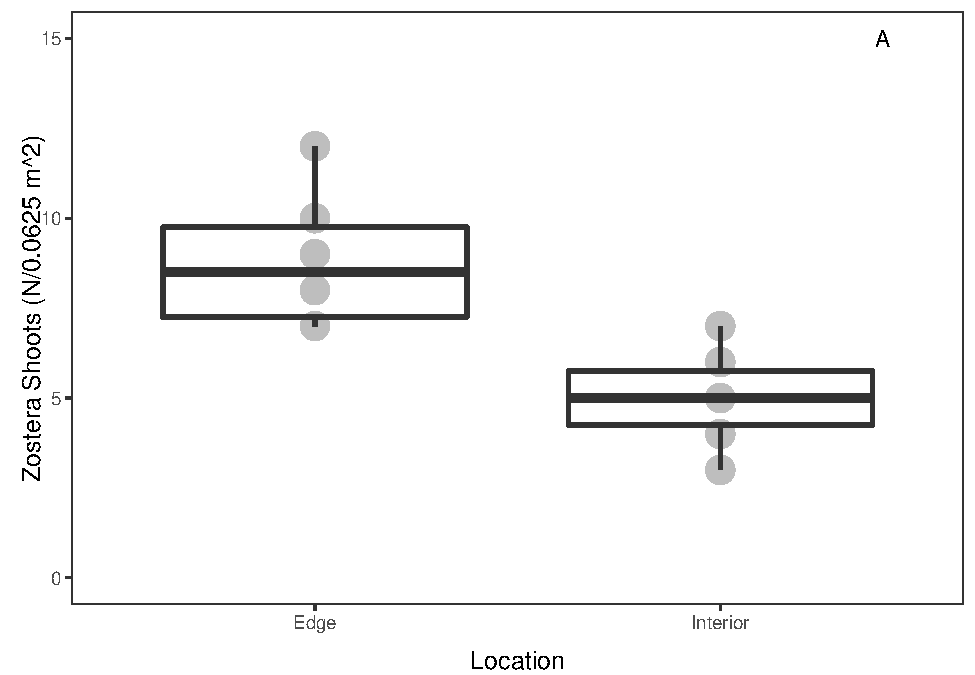
\includegraphics{Griffiths_et_al_analyses_and_figures_files/figure-latex/unnamed-chunk-7-1.pdf}

\section{Analysis}\label{analysis}

\begin{verbatim}
## Analysis of Variance Table
## 
## Response: number.shoots.quadrat
##           Df Sum Sq Mean Sq F value   Pr(>F)   
## site       1 44.083  44.083  15.289 0.002913 **
## Residuals 10 28.833   2.883                    
## ---
## Signif. codes:  0 '***' 0.001 '**' 0.01 '*' 0.05 '.' 0.1 ' ' 1
\end{verbatim}

\begin{enumerate}
\def\labelenumi{\Alph{enumi})}
\tightlist
\item
  Zostera shoot density
  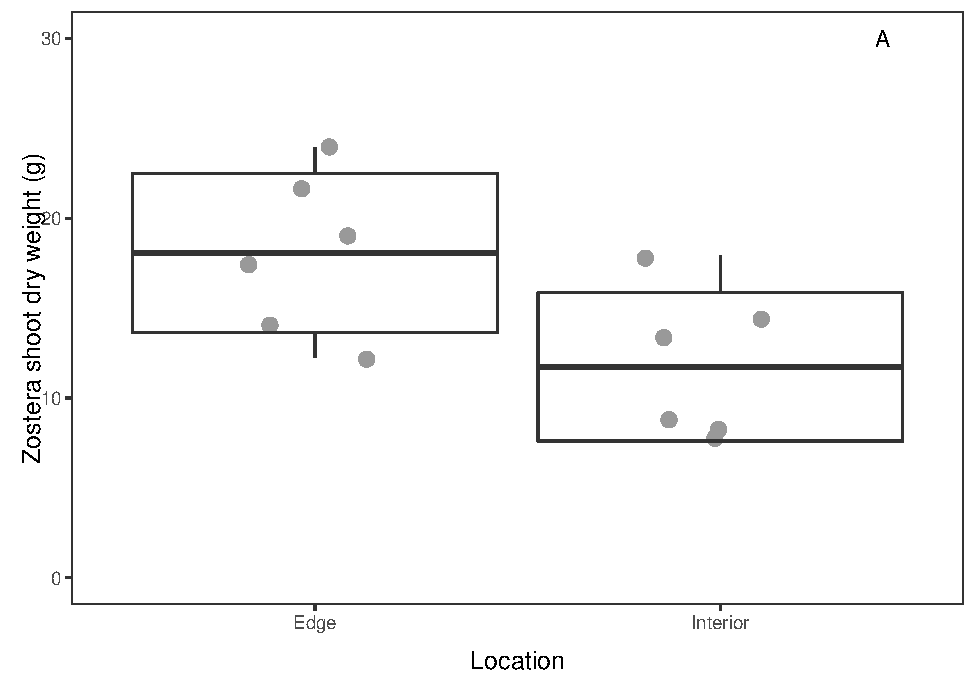
\includegraphics{Griffiths_et_al_analyses_and_figures_files/figure-latex/unnamed-chunk-9-1.pdf}
\end{enumerate}

Zostera above ground dry weight

\begin{verbatim}
## Analysis of Variance Table
## 
## Response: total.dry.macro.weight
##           Df Sum Sq Mean Sq F value Pr(>F)  
## site       1 119.76 119.764  6.5721 0.0282 *
## Residuals 10 182.23  18.223                 
## ---
## Signif. codes:  0 '***' 0.001 '**' 0.01 '*' 0.05 '.' 0.1 ' ' 1
\end{verbatim}

\begin{enumerate}
\def\labelenumi{\Alph{enumi})}
\setcounter{enumi}{1}
\item
  Smithora load (dry weight)
  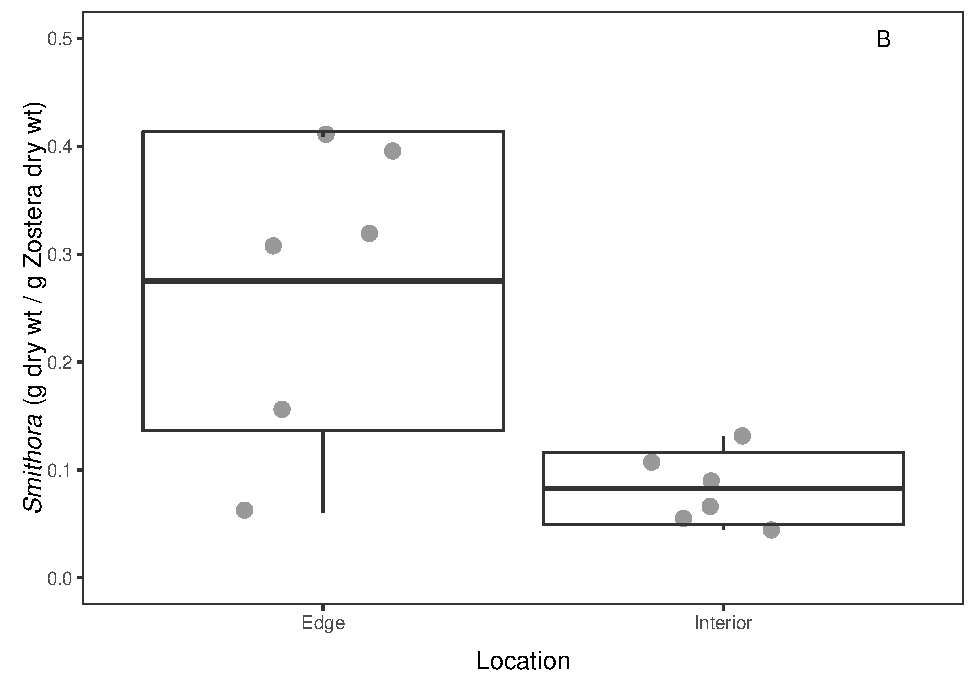
\includegraphics{Griffiths_et_al_analyses_and_figures_files/figure-latex/unnamed-chunk-11-1.pdf}
\item
  GRAZER ABUNDANCE -- placeholder, waiting for final plot labels from
  Gwen
\end{enumerate}

\begin{verbatim}
## Warning: Removed 1 rows containing missing values (geom_boxplot).
\end{verbatim}

\includegraphics{Griffiths_et_al_analyses_and_figures_files/figure-latex/unnamed-chunk-12-1.pdf}

\begin{verbatim}
## Warning: Removed 1 rows containing missing values (geom_boxplot).
\end{verbatim}

FIGURE 3: Smithora results post experiment - remake this figure. april
5th: i'm not if it still needs to be remade - i have to check this.
\includegraphics{Griffiths_et_al_analyses_and_figures_files/figure-latex/unnamed-chunk-13-1.pdf}

Experimental analysis:

first analyze control vs unmanipulated
\includegraphics{Griffiths_et_al_analyses_and_figures_files/figure-latex/unnamed-chunk-14-1.pdf}

\begin{verbatim}
## Analysis of Variance Table
## 
## Response: (smith.expt[(smith.expt$Type != "Transplanted"), ]$ratio)
##                                                          Df  Sum Sq
## smith.expt[(smith.expt$Type != "Transplanted"), ]$Type    1 0.04611
## smith.expt[(smith.expt$Type != "Transplanted"), ]$Source  1 0.76559
## Residuals                                                10 0.29064
##                                                          Mean Sq F value
## smith.expt[(smith.expt$Type != "Transplanted"), ]$Type   0.04611  1.5863
## smith.expt[(smith.expt$Type != "Transplanted"), ]$Source 0.76559 26.3415
## Residuals                                                0.02906        
##                                                             Pr(>F)    
## smith.expt[(smith.expt$Type != "Transplanted"), ]$Type   0.2364526    
## smith.expt[(smith.expt$Type != "Transplanted"), ]$Source 0.0004426 ***
## Residuals                                                             
## ---
## Signif. codes:  0 '***' 0.001 '**' 0.01 '*' 0.05 '.' 0.1 ' ' 1
\end{verbatim}

then analyze control v transplanted
\includegraphics{Griffiths_et_al_analyses_and_figures_files/figure-latex/unnamed-chunk-15-1.pdf}

\begin{verbatim}
## Analysis of Variance Table
## 
## Response: log(smith.expt[(smith.expt$Type != "Unmanip."), ]$ratio + 1)
##                                                                                                         Df
## smith.expt[(smith.expt$Type != "Unmanip."), ]$Type                                                       1
## smith.expt[(smith.expt$Type != "Unmanip."), ]$Source                                                     1
## smith.expt[(smith.expt$Type != "Unmanip."), ]$Type:smith.expt[(smith.expt$Type != "Unmanip."), ]$Source  1
## Residuals                                                                                               11
##                                                                                                          Sum Sq
## smith.expt[(smith.expt$Type != "Unmanip."), ]$Type                                                      0.00346
## smith.expt[(smith.expt$Type != "Unmanip."), ]$Source                                                    0.39377
## smith.expt[(smith.expt$Type != "Unmanip."), ]$Type:smith.expt[(smith.expt$Type != "Unmanip."), ]$Source 0.05737
## Residuals                                                                                               0.13517
##                                                                                                         Mean Sq
## smith.expt[(smith.expt$Type != "Unmanip."), ]$Type                                                      0.00346
## smith.expt[(smith.expt$Type != "Unmanip."), ]$Source                                                    0.39377
## smith.expt[(smith.expt$Type != "Unmanip."), ]$Type:smith.expt[(smith.expt$Type != "Unmanip."), ]$Source 0.05737
## Residuals                                                                                               0.01229
##                                                                                                         F value
## smith.expt[(smith.expt$Type != "Unmanip."), ]$Type                                                       0.2813
## smith.expt[(smith.expt$Type != "Unmanip."), ]$Source                                                    32.0436
## smith.expt[(smith.expt$Type != "Unmanip."), ]$Type:smith.expt[(smith.expt$Type != "Unmanip."), ]$Source  4.6684
## Residuals                                                                                                      
##                                                                                                            Pr(>F)
## smith.expt[(smith.expt$Type != "Unmanip."), ]$Type                                                      0.6064020
## smith.expt[(smith.expt$Type != "Unmanip."), ]$Source                                                    0.0001465
## smith.expt[(smith.expt$Type != "Unmanip."), ]$Type:smith.expt[(smith.expt$Type != "Unmanip."), ]$Source 0.0536429
## Residuals                                                                                                        
##                                                                                                            
## smith.expt[(smith.expt$Type != "Unmanip."), ]$Type                                                         
## smith.expt[(smith.expt$Type != "Unmanip."), ]$Source                                                    ***
## smith.expt[(smith.expt$Type != "Unmanip."), ]$Type:smith.expt[(smith.expt$Type != "Unmanip."), ]$Source .  
## Residuals                                                                                                  
## ---
## Signif. codes:  0 '***' 0.001 '**' 0.01 '*' 0.05 '.' 0.1 ' ' 1
\end{verbatim}


\end{document}
